\section{Astrophysical Example}

\begin{figure*}
  \centering
  \vspace{-0.5cm}
  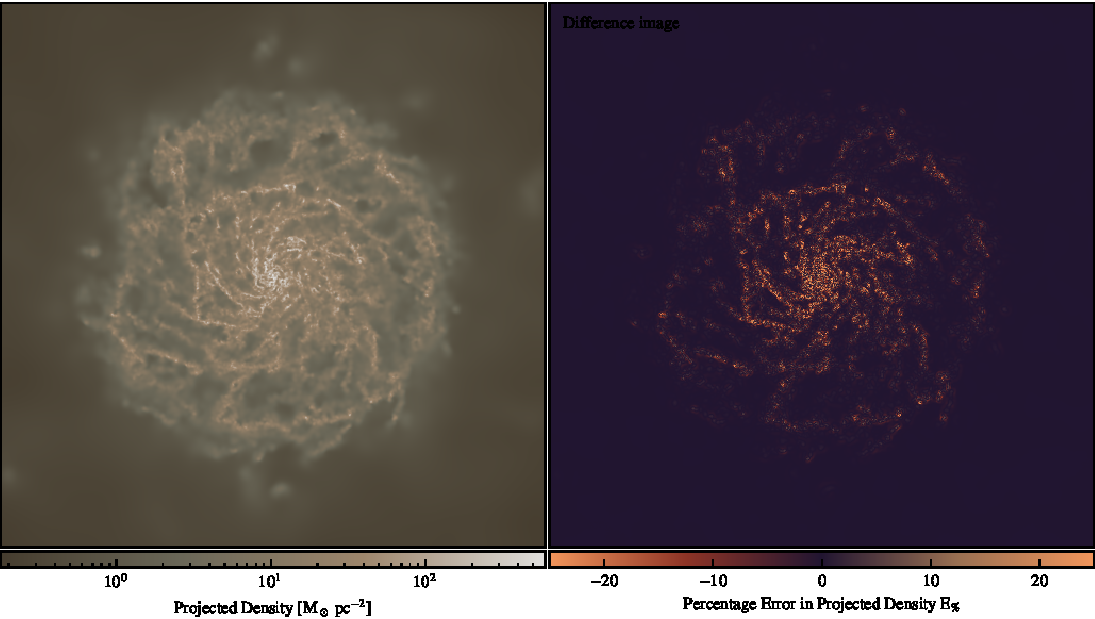
\includegraphics[width=\textwidth]{./plots/galaxy/error_image.pdf}
    \caption{\emph{Left:} Projected (`surface') density of a spiral galaxy from an SPH simulation performed with {\tt SWIFT}. The projected density was calculated on a 512$^2$ grid, with each pixel corresponding to 100 pc of physical space, a common size in observations of real galaxies. \emph{Right:} The error in the estimation of the surface density when not subsampling particles close to, or smaller than, the grid size (i.e. using the `Original' algorithm). This correlates with medium-high density regions of the galaxy, where many particles have smoothing lengths below the grid size. Note that 1 pc = $3.09 \times 10^{16}$ m.}
  \label{fig:error_image}
\end{figure*}


\begin{figure}
  \centering
  \vspace{-0.25cm}
  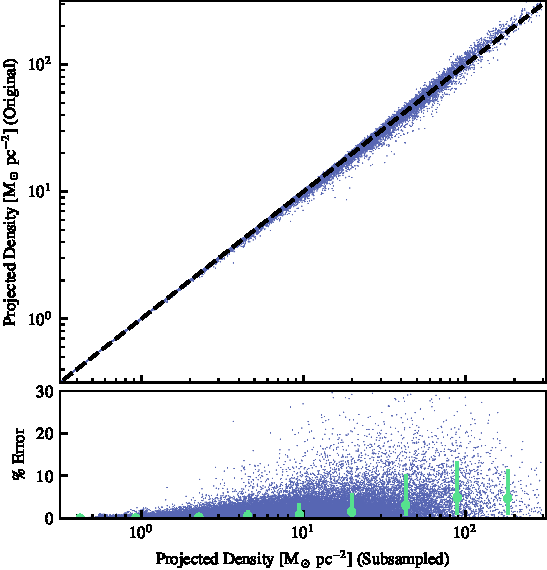
\includegraphics[width=\columnwidth]{./plots/stellar/surface_density_comparison.pdf}
    \caption{Comparison of projected density calculated with the subsampled strategy (horizontal) and original (vertical) algorithm, for the galaxy in Fig. \ref{fig:error_image}. The black dashed line shows the 1:1 relation. The bottom panel shows the percentage error, with each point corresponding to an individual pixel and the green points corresponding to the 10th, 50th, and 90th percentile (bottom, point, and top of bar) in ten bins across the sampled surface density range.}
  \label{fig:sdcomparison}
  \vspace{-0.15cm}
\end{figure}

So far we have only considered the impact of the subsampling technique on simple problems, but have already demonstrated its ability to provide highly accurate, converged, solutions at all grid sizes. We now consider the astrophysical example of an isolated galaxy disk. The properties of galaxies are the key discriminator between galaxy formation models, as they host an abundance of readily observable properties which can be directly compared with projected quantities from SPH simulations.

This galaxy was simulated with the {\tt SWIFT} code, using the \textsc{Sphenix} \cite{Borrow2020c} hydrodynamics model, and an analytical Hernquist \cite{Hernquist1990} potential for the dark matter component with a mass of $M_{200} = 1.37\times 10^{12}$ M$_\odot$ with M$_\odot = 2\times10^{30}$ kg, concentration $c=9.0$, and a disk fraction of $4\%$. The simulation contains 123533 directly simulated gas particles (of mass $10^5$ M$_\odot$), which interact both through hydrodynamics and gravity, and 424467 star particles (of mass $10^5$ M$_\odot$) that only interact gravitationally. All particles are subject to a modified version of the EAGLE sub-grid model \cite{Schaye2015}, which includes prescriptions for radiative cooling \cite{Ploeckinger2020}, star formation \cite{Schaye2008}, and stellar feedback \cite{DallaVecchia2012}. Here we use a snapshot after $t=0.5$ Gyr, with 1 Gyr $= 3.16\times10^{16}$ s. The initial conditions set-up is described in more detail as the {\tt fid} galaxy in \cite{Schaye2008}. 

Fig. \ref{fig:error_image} shows the projected gas density of the galaxy in the left panel and the percentage error attained from such a projection if using the original scheme. The pixels are set to be 100 pc on a side, for comparison with typical observations of real galaxies (e.g. \cite{Bigiel2008}). The dynamic range in smoothing length here is 300, with $h_{\rm min} = 33$ pc. Here, the percentage error is calculated relative to the subsampled result for more consistent and simple visualisation in later figures, but the result is unchanged when comparing to a high resolution downsampled grid.

The higher density regions of the galaxy (near to the centre) do not have the largest errors due to the stacking of particle layers; this simulation was performed in three dimensions, and as such the Monte Carlo-style sampling is less poor than when only a single layer of particles is considered. In the intermediate density regions, where there is also a strong gradient in density, the error spikes as the kernel gradients are poorly resolved without subsampling. This is a particularly dangerous error structure, as it is typically assumed that the error in SPH simulations decreases as the density increases and the finite mass sampling of the field improves. 

\begin{figure}
  \centering
  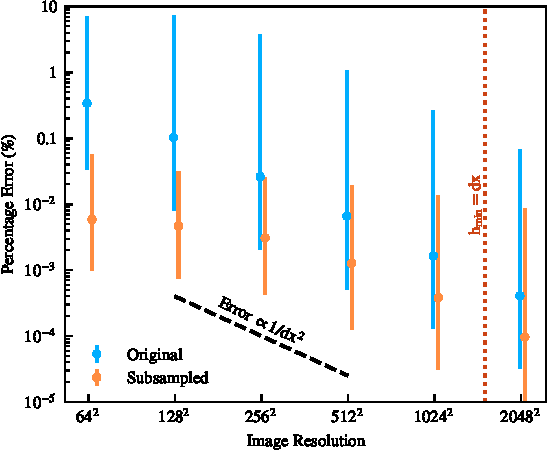
\includegraphics[width=\columnwidth]{./plots/galaxy/test_convergence.pdf}
  \caption{Compares the errors (in the 10\%, 50\%, 90\% percentiles from bottom, point, to top) for the original and subsampled method for the isolated galaxy in Fig. \ref{fig:error_image}. Note that each point is evaluated at the number of pixels given on the horizontal axis, with them offset for clarity when the range bars overlap.}
  \label{fig:galconv}
\end{figure}

The density-dependent error findings are confirmed in Fig. \ref{fig:sdcomparison}, where the projected densities in individual pixels are compared between the two methods. The increase in error with density, except at the highest densities, is confirmed. Additionally, the error is not biased or systematic in any way; the errors inherent in using the poorly sampled projection method are random and as such impossible to offset with, for instance, a scaling factor. 

Fig. \ref{fig:galconv} shows the convergence of the median error with image resolution. Because of the higher dynamic range in this image, relative to the gradient in Fig. \ref{fig:gradconv}, the error ranges for both methods are larger. Here we see that the subsampled method provides a lower than $0.1\%$ error for all pixels, with the original method, as demonstrated in Fig. \ref{fig:sdcomparison}, leading to errors for individual pixels that are higher than 30\%. The median error does converge at the expected rate, but as noted before as real-world observations are taken on coarse grids the convergence properties are not relevant to the accuracy of the method.

These final two figures demonstrate that the correct sampling of kernels in projection is not simply an academic exercise; for simulated observations of real-world problems in adaptive environments subsampling is necessary to produce accurate results.